% !TEX root =  main.tex

%Description of \m\mEdhoc and main changes from last verified version

\vnote{I find the macros for the protocol, method, and tool names distracting while reading through (the font changes too much, too often). The macro for EDHOC actually inserts a line break if you start a sentence with it, because of the \texttt{hbox} (I'm not sure why the hbox exists for what is a macro to be inserted in running text). I do need to start sentence with EDHOC many times though, so this is irritating. It is also the case that ProVerif needs to be written like so, and not capitalized entirely, so at least one of them is plain wrong! For now I've left in the macros, but I'd prefer that we fixed them to be regular capitalized text or, in the case of ProVerif, in camelcase as they should be.}

\subsection{Overview}
Constrained IoT systems often deal with a lot of valuable personal and business information that ought to be kept secure. Such systems need to be assured of end-to-end protection with source authentication and perfect forward secrecy. It is often desirable to protect such devices at the application layer -- for example, in cases where transport layer security is not sufficient [\mcneed], or where multiple underlying protocols need to be accounted for. One method for providing application layer security is provided by CBOR Object Signing and Encryption (COSE) [RFC8152: \mcfix].  

In order to derive shared key material with which to proceed, communicating parties can run an Elliptic Curve Diffie-Hellman key exchange protocol with ephemeral keys. Ephemeral Diffie-Hellman Over COSE (\mEdhoc) is a lightweight key exchange protocol for such situations, and is expected to provide perfect forward secrecy and identity protection. \mEdhoc supports authentication using pre-shared keys (PSK), raw public keys (RPK), and public key certificates. After successful completion of the \mEdhoc protocol, application keys and other application specific data can be derived using the \mEdhoc-Exporter interface. 

A main use case for \mEdhoc is to establish a security context for Object Security for Constrained RESTful Environments (\mOscore) [RFC8613: \mcfix]. \mOscore is a protocol which uses COSE for application-layer protection on top of the transport-layer Constrained Application Protocol (CoAP). \mEdhoc uses COSE for cryptography, CBOR for encoding, and CoAP for transport. By reusing existing libraries, the additional code footprint can be kept very low.

\mEdhoc is designed to work in highly constrained scenarios. This makes it especially suitable for network technologies which have low throughput, low power consumption, and small frame sizes. Examples include Cellular IoT, 6TiSCH, and LoRaWAN [\mcneed].

\subsection{Background, comparison with~\cite{DBLP:conf/secsr/BruniJPS18}}
The first version of \mEdhoc was proposed in March 2016 to a working group investigating lightweight authenticated key exchange protocols [\mcneed]. There has been a focus on formally verifying that the protocol satisfies the properties expected of it right from the beginning. 

The 2018 work~\cite{DBLP:conf/secsr/BruniJPS18} by Bruni et al performed a formal verification of version 08 [\url{https://tools.ietf.org/html/draft-selander-ace-cose-ecdhe-08} \mcfix] of \mEdhoc. The protocol and properties are modelled and verified in the \mProverif tool. This version of the protocol belongs to the \mSigmaI family of protocols, and has two modes -- one with asymmetric keys, and one with pre-shared symmetric keys (PSK). Bruni et al showed that this version satisfies the requisite properties of identity protection, (perfect forward) secrecy of data, and strong authentication, upon completion of the protocol.

\mEdhoc has undergone a lot of change since version 08, as will be described in the following sections, and the formal verification of the current version, therefore, is a worthwhile exercise.

%\subsection{Overarching goal of security context establishment}
\section{Methods and features of \textsc{EDHOC}}
\mEdhoc can established Diffie-Hellman key exchange in one of three different ways -- using digital signatures, static Diffie-Hellman keys, or pre-shared symmetric keys. We describe each of these methods in detail below. The communicating parties must agree on the method and cipher suite used for encryption as part of the first message. The parties exchange ephemeral public keys, compute the shared secret, and derive symmetric application keys from this secret.

\vnote{Need a quick and dirty introduction to COSE here}

\subsection{\mPskPsk method}
In this method, the initiator and responder are assumed to have a pre-shared key which is secret to them, and can be retrieved by the responder using a public part of the first message (\mIDPSK). This method corresponds to the symmetric key method of \mEdhoc v08. 

In the first message, the initiator sends a message consisting of the method name, the cipher suites ranked in order of preference, the initiator's ephemeral key (\mGx), their connection identifier (\mCi), the \mIDPSK identifier, and (optional) auxiliary data (\mADone). The responder, upon receipt of this message, must verify that the selected cipher suite is supported,  and pass \mADone to the security application which needs it. If any verification step fails, the initiator sends an EDHOC error message back, and the protocol aborts.

The second message, sent by the responder, is composed of \mCi, the responder's ephemeral key \mGy, their connection identifier \mCr, and a COSE object. This contains as external data the transaction hash of the first message (\mTHtwo), along with an AEAD encryption [\mcneed] of the (optional) auxiliary data \mADtwo. The key used for this (\mKtwo) is derived using the EDHOC key derivation function with \mTHtwo and the pseudorandom string \mPRKtwo as input, while the associated data for the AEAD encryption is constructed by concatenating a constant string, plaintext \mhplain, and \mTHtwo. 

The initiator, upon receipt of this message, sends back \mCr, followed by a COSE object containing an AEAD encryption of auxiliary data \mADthree, along with the transaction hash of the second message (\mTHthree) as external data. As earlier, the key used is derived by supplying \mTHthree and \mPRKthree as input to the KDF, and the associated data obtained by concatenating the constant string, plaintext \mhplain, and \mTHthree. An abstract description is shown in Figure~\ref{fig:edhocpsk}.

\vnote{Figure numbers don't square up, check class file guidelines!}

\begin{figure}[!h]\label{fig:edhocpsk}
\centering
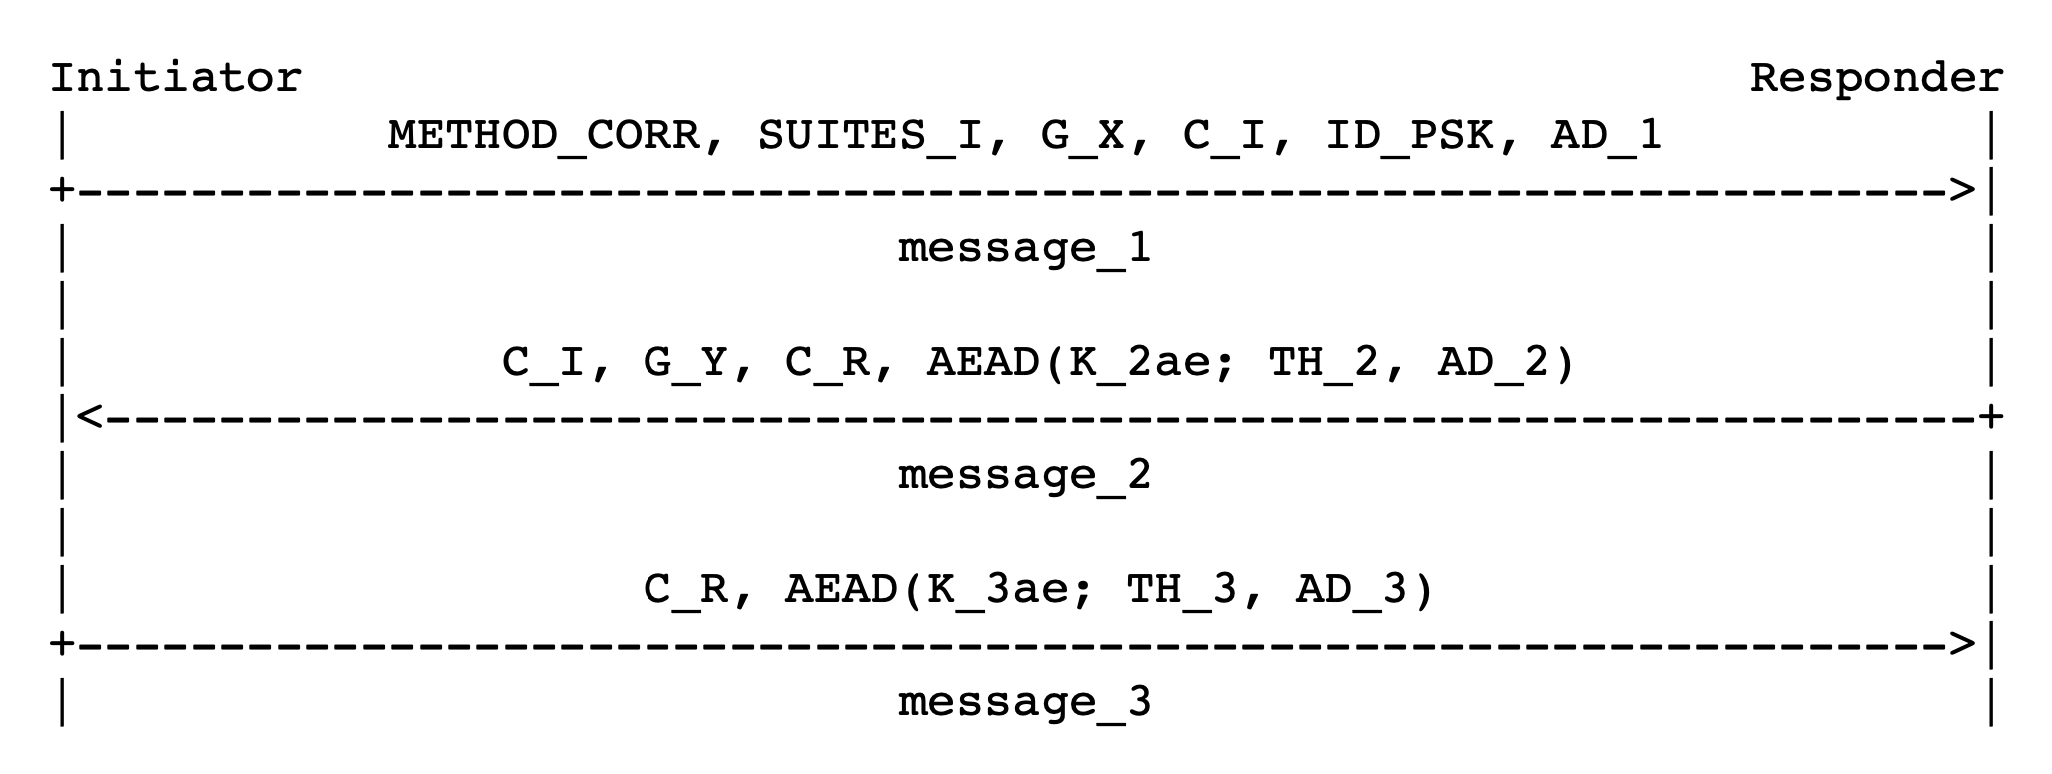
\includegraphics[scale=0.3]{Images/psk.png}
\caption{The PSK-PSK method of EDHOC}
\end{figure}

\subsection{\mStat-based methods}
\mEdhoc allows for three \mStat-based methods -- two where only one participant has a static Diffie-Hellman key (while the other uses signatures), and one where both do. This set of methods is not covered in previous versions of \mEdhoc, which only has a single \mSigma asymmetric key method (corresponding to the \mSigSig method shown above). This allows one party to use a \mSigma style of authentication using signatures, while the other can use static DH keys, along the lines of \mOptls. In Figure~\ref{fig:edhocasym}, a template for all the asymmetric key methods of EDHOC is shown. 

\begin{figure}[!h]\label{fig:edhocasym}
\centering
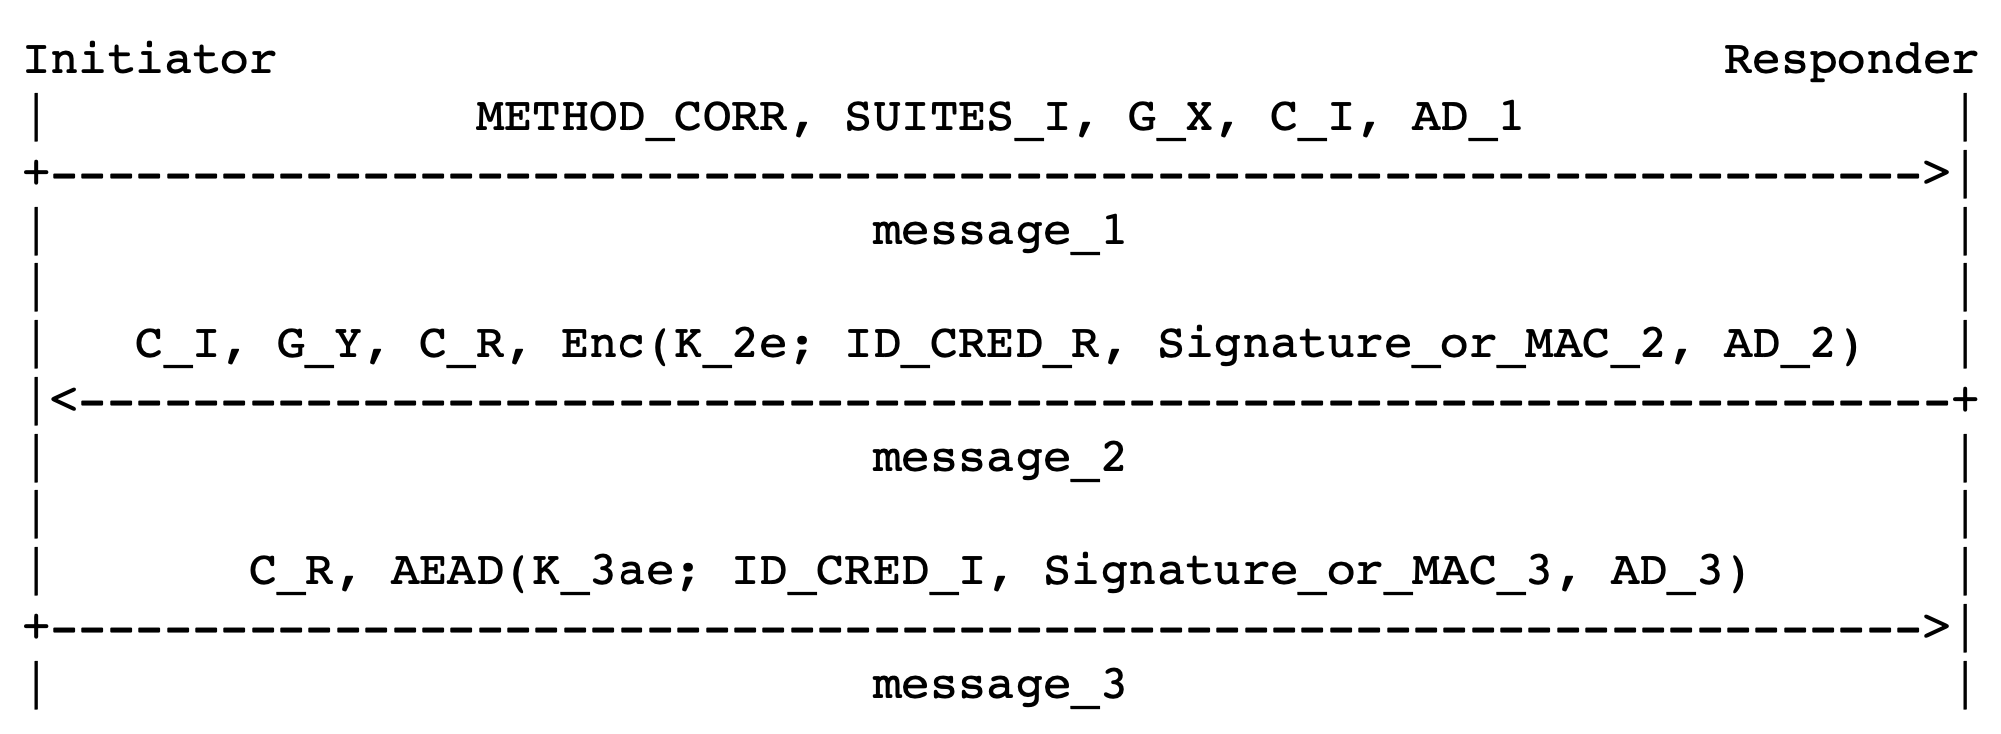
\includegraphics[scale=0.3]{Images/asym.png}
\caption{A template for the asymmetric key methods of EDHOC}
\end{figure}

In the first message, the initiator includes an identifier for the method, a preference-ordered list of cipher suites, their ephemeral key \mGx, their connection identifier \mCi, and some optional plaintext \mADone. This message is common to all the four methods below involving asymmetric keys. 

The responder, upon receipt, verifies the cipher suites, passes any \mADone to the application that needs it, and proceeds to construct and send the second message. This message contains (not necessarily all of) \mCi, \mGy, \mCr, and an encrypted term. The initiator, upon getting this message, sends out a message containing an encrypted term. Depending on the methods being run by the initiator and responder, the exact contents of these messages may vary. We will now describe each of these methods and the second and third messages therein in detail.

\subsubsection{\mSigStat}
The initiator runs a \mSigma-based method, with signatures, while the responder operates with a static Diffie-Hellman key and MACs. Since this method is one where the responder runs \mStat, in the second message, \mCi is omitted. The encrypted term for the second message is constructed as follows. 

First, we build the COSE object that is the inner MAC, since the responder runs \mStat. The protected part of this object is an identifier for retrieving the responder's public authentication key \mCredr. The externally supplied data is the transaction hash \mTHtwo of the first message and \mGy,  the responder's public authentication key \mCredr, and (optional) auxiliary data \mADtwo. The key used for the encryption is the output of the KDF on being fed as input the pseudorandom string \mPRKthree and \mTHtwo. The resulting encrypted object is now referred to as the ciphertext \mMactwo. 

For the outer encryption object, we consider the plaintext formed by concatenating the bitstrings corresponding to the identifier for \mCredr, \mMactwo, and \mADtwo (if any). The encryption is obtained by performing an \mXor operation on this plaintext with the key \mKtwo, which is obtained by using the KDF on \mPRKtwo and the transaction hash \mTHtwo. The responder therefore sends to the initiator \mGy, \mCr, and this COSE encryption object as the second message.

The initiator responds with the third message, consisting of \mCr, and an encrypted object. Here, again, we first build the inner COSE object. This process is analogous to that employed by the responder for the second message. The COSE object has as protected data an identifier for retrieving the initiator's public authentication key \mCredi. The externally supplied data is the transaction hash \mTHthree of the second message and \mTHtwo,  the initator's public authentication key \mCredi, and (optional) auxiliary data \mADthree. The key used is obtained by inputing the pseudorandom string \mPRKfour and \mTHthree. The resulting encrypted object is now referred to as the ciphertext \mMacthree. 

Since the initiator is running \mSig, this COSE object needs to be signed. To the signing algorithm, the initiator sends as protected data the identifier for retrieving \mCredi, as external data the concatenation of \mTHthree, \mCredi, and any \mADthree, and \mMacthree. This is signed using the private authentication key of the Initiator.  

We now construct the encryption for the third message, by passing to an AEAD encryption algorithm a COSE object with no protected data, external data \mTHthree, and a plaintext obtained by concatenating the identifier for retrieving \mCredi, the signed object described above, and \mADthree. The key used for encryption is \mKthree, obtained by running the KDF on the pseudorandom string \mPRKthree and \mTHthree. Thus, the message sent by the initiator to the responder in the third step is \mCr accompanied by this encrypted object.

\vnote{Need to insert tikZ figures}

\subsubsection{\mStatStat}
In this method, both the initiator and the responder run the \mStat method. The responder's message looks exactly the same as in the previous subsection, for \mSigStat. The initiator's message, however, is not signed anymore, since the initiator too is running the \mStat method. Thus, we skip the signature process in the steps described above, and instead of passing a signed object to the AEAD encryption algorithm, we pass \mMacthree itself. Everything else stays the same as earlier.

\subsubsection{\mStatSig}
Here, the responder runs the \mSig method, while the initiator runs the \mStat method. 

\vnote{Need to talk about links to OPTLS and NOISE here or later?}

\subsection{\mSigSig method}
The \mSigma (SIGn-and-MAc) family of protocols [\mcneed] has many variants. The \mSigSig method of \mEdhoc is built on \mSigmaI, a variant of the \mSigma protocol which provides identity protection for the initiator, and  implements the \mSigmaI variant as Mac-then-Sign. The current \mSigSig method corresponds (with a few minor changes) to the asymmetric key mode of \mEdhoc v08. 




\subsection{Expected security properties}


%Discussion of KDF -- page 13 of EDHOC

%certain security applications may be integrated into EDHOC by transporting auxiliary data together with the messages. One example is the transport of third-party authorization information protected outside of EDHOC [I-D.selander-ace-ake-authz]. Another example is the embedding of a certificate enrolment request or a newly issued certificate. EDHOC allows opaque auxiliary data (AD) to be sent in the EDHOC messages. Unprotected Auxiliary Data (AD_1, AD_2) may be sent in message_1 and message_2, respectively. Protected Auxiliary Data (AD_3) may be sent in message_3. Since data carried in AD1 and AD2 may not be protected, and the content of AD3 is available to both the Initiator and the Responder, special considerations need to be made such that the availability of the data a) does not violate security and privacy requirements of the service which uses this data, and b) does not violate the security properties of EDHOC. 

